%%________________________________________________________________________
%% LEIM | PROJETO
%% 2022 / 2013 / 2012
%% Modelo para relatório
%% v04: alteração ADEETC para DEETC; outros ajustes
%% v03: correção de gralhas
%% v02: inclui anexo sobre utilização sistema controlo de versões
%% v01: original
%% PTS / MAR.2022 / MAI.2013 / 23.MAI.2012 (construído)
%%________________________________________________________________________


%%________________________________________________________________________
\chapter{Implementação do Modelo}
\label{ch:implementacaoDoModelo}
%%________________________________________________________________________

Neste capítulo iremos descrever de forma detalhada como foi feita a transição do modelo proposto para a implementação  da aplicação. A abordagem seguida foi iterativa, com várias fases de experimentação e validação, sempre em articulação com os objetivos definidos para o projeto e os dados reais obtidos anteriormente.

Começamos por abordar o processo de análise e classificação dos dados, uma vez que a estrutura e qualidade da informação recebida tiveram um impacto direto na forma como os dados seriam processados, armazenados e, mais tarde, visualizados. A seguir, exploramos a construção do pipeline de transformação, a lógica de organização dos ficheiros e o modo como garantimos que cada carregamento fosse tratado de forma automática. Por fim, explicamos as decisões que nos levaram à escolha de representações gráficas específicas, assim como os mecanismos que permitem ao utilizador interagir com os dados.

\section{Análise dos dados}

O processo de análise começou após a reunião inicial comm os orientadores do projeto, onde recebemos os ficheiros com que iamos trabalhar. Tratar este ficheiros implicou várias fases de análise, onde delineamos estratégias para conseguir extrair dados e possiveis gráficos. Antes de falarmos das várias fases, teremos só de estabelecer que tipos de gráficos são os indicados para as informações que queremos mostrar.

\subsection{Análise inicial da informação}
\label{sec:analiseInicial}

Após termos recebido os dados, fizemos uma primeira análise com o objetivo de perceber a informação recebida e os próximos passos a tomar.

No total, recebemos 30 ficheiros \gls{xlsx} que foram exportados da plataforma, correspondentes às diferentes secções da plataforma de simulação, com vários indicadores como segmentos de mercado, características de produto, vendas, entre outros. Cada ficheiro pode conter várias folhas de cálculo, que no total são 103 folhas de cálculo, organizadas por marcas, cidades entre outros marcadores.

Durante esta análise preliminar, verificámos que:
\begin{itemize}
    \item Os nomes dos ficheiros e das folhas variam, mas seguem uma estrutura relativamente consistente;
    \item Alguns ficheiros apresentam estruturas de dados semelhantes, mas com diferenças no nível de detalhe ou na organização das colunas e linhas;
    \item Existiam ficheiros com dados que iriam precisar de mais transformação uma vez que representavam vários tipos de unidades (como por exemplo percentagens, valores monetários, valores relativos, etc) na mesma folha de cálculo;
    \item Dados com muito detalhe, e com várias colunas sem representação (células marcadas com "X", linhas com valores nulos e fundo amarelo).
\end{itemize}

Com base nesta primeira análise, concluímos que seria necessário:
\begin{itemize}
    \item Fazer uma normalização da informação recebida para garantir uma utilização consistente da aplicação;
    \item Separar os vários ficheiros possiveis em grupos, de forma a identificar dados em comum que pudéssemos aplicar \textit{templates} de gráfico;
    \item Guardar os dados extraídos num formato mais prático, e que permita uma filtragem dinâmica da informação carregada (de forma a facilitar a visualização dos dados)-
    \item Em algumas séries de dados, identificamos colunas que se podiam remover devido a serem redundantes, ou por representarem informação que já é representada por outras colunas (como por exemplo colunas de valores totais ou outras discutidas com os orientadores);
\end{itemize}

Esta análise inicial permitiu-nos estabelecer as fases seguintes em relação ao tratamento que iremos dar aos vários ficheiros possiveis. Para isso, decidimos classificar a informação em várias categorias, e aplicar tipos de gráficos especificos a cada categoria, tendo assim \textit{templates} que podemos aplicar programaticamente. 

\subsection{Classificação da informação}

A análise inicial dos ficheiros fornecidos permitiu-nos perceber que, apesar da diversidade dos mesmos,  existiam padrões consistentes na estrutura. Com base nisso, tomámos a decisão de agrupar os ficheiros em \textit{buckets} ou categorias lógicas. Cada um desses grupos ficou associado a um \textit{template} gráfico específico, o que nos permite não só uniformizar a apresentação dos dados, como também automatizar o processo de transformação e visualização a partir dos ficheiros.

Os grupos definidos foram os seguintes: \textbf{simples}, \textbf{agrupado}, \textbf{balanços}, \textbf{quartis}, \textbf{setores} e \textbf{análise específica}. Vamos então descrever o significado de cada grupo e identificar o que é comum entre os gráficos pertencentes a cada um deles.

O grupo \textbf{simples} inclui ficheiros cuja estrutura é mais direta, geralmente com apenas duas colunas: uma coluna que representa uma categoria (como por exemplo empresas ou segmentos de mercado) e uma coluna numérica (como por exemplo vendas ou lucros). Nestes casos, optámos por gráficos de barras, uma vez que o objetivo principal é comparar rapidamente valores individuais entre categorias. Nos ficheiros que avaliamos, não encontramos séries temporais, pelo que não justificou gráficos de linhas. Também nesta categoria, alguns dados eram séries mais específicas (como dados relativos a médias e medianas) mas mantinham a mesma estrutura de dados, pelo que foram classificados como \textbf{simples} mas utilizaram gráficos diferentes como gráficos de diagramas e quartis e gráficos de setores (também conhecidos como \textit{pie charts}).

O grupo \textbf{duplo} refere-se a ficheiros onde existem múltiplas séries de dados associadas à mesma categoria. Ou seja, para cada categoria, existem vários valores (ou várias séries) que precisam de ser representados lado a lado. Para estes casos, a escolha que fizemos foi apresentar gráficos de barras agrupadas, permitindo uma comparação direta entre diferentes séries de dados para a mesma categoria, e permite visualizar todos os dados relacionados com essa categoria.

O grupo \textbf{balanços} abrange ficheiros associados a balanços financeiros ou variações de stock, onde faz sentido representar aumentos e diminuições de valores ao longo de um processo ou período. Para estes ficheiros, o \textit{template} selecionado foi o gráfico de cascata (ou um gráfico \textit{financial waterfall}), dado que este tipo de visualização representa as várias componentes do valor total.

No grupo \textbf{quartis}, classificámos ficheiros onde os dados contem minimos, máximos e médias. Aqui, optámos por representar a informação através de gráficos de quartis, que são uteis para mostrar a mediana, a dispersão e possíveis valores \textit{outliers}. Para este tipo de gráfico, tentámos sempre fazer com que a leitura do mesmo seja o mais fácil possível.

O grupo \textbf{setores} inclui ficheiros onde a segmentação do mercado ou da performance está organizada por setores económicos ou geográficos. Nestes casos, faz sentido usar gráficos de setores (também conhecidos como \textit{pie charts}),  dependendo da necessidade de comparar proporções entre segmentos.

Finalmente, o grupo de \textbf{análise específica} são ficheiros que não se encaixam diretamente nos formatos anteriores, como análises mais detalhadas por cidade, por segmento ou quando os dados incluem várias unidades na mesma folha (percentagens com euros). Para estes casos, o processo passou por simplificar a informação de modo a encaixar num dos grupos acima ou excecionalmente aplicar um novo tipo de gráfico, e a análise foi feita manualmente para cada caso. Para casos em que a não era possível aplicar um \textit{template} de gráfico, não foi possivel simplificar a informação e não encontrámos uma representação gráfica que fosse fácil de interpretar, optámos por não aplicar nenhum gráfico, e apenas apenas mostrar uma tabela interativa com os dados onde o utilizador podia filtrar os dados por diferentes colunas.


No final, dos 30 ficheiros recebidos, a classificação foi a seguinte:
\begin{figure}[h]
    \centering
    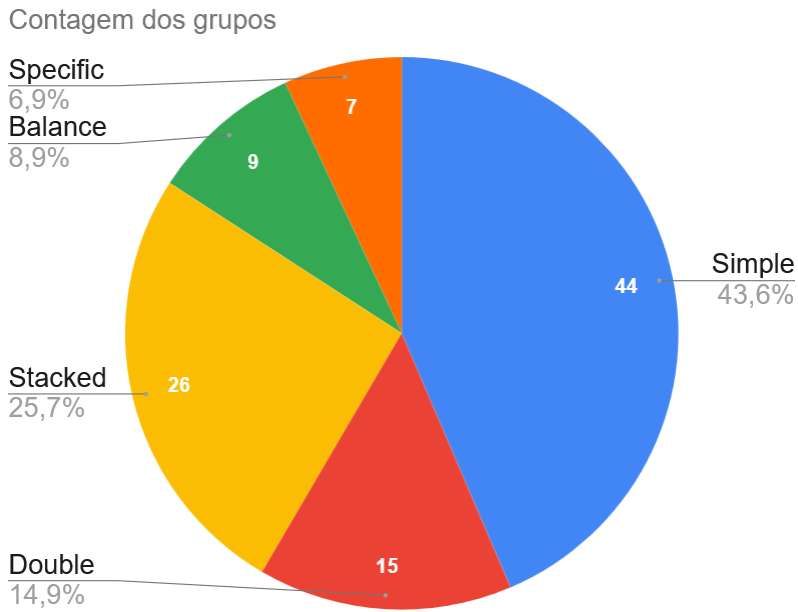
\includegraphics[width=\textwidth]{./img/stats1}
 \caption{Classificação dos ficheiros - contagem final dos grupos}
 \end{figure}

Em termos de representações utilizadas, a distribuição é a seguinte:
\begin{figure}[h]
    \centering
    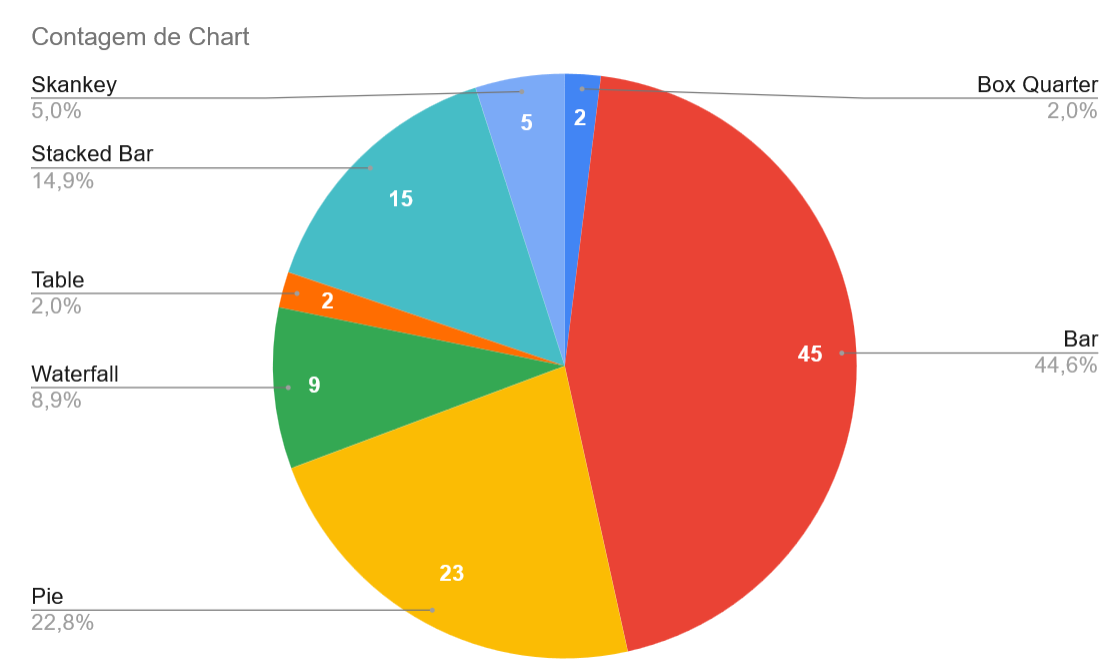
\includegraphics[width=\textwidth]{./img/stats2}
 \caption{Classificação dos ficheiros - contagem final de representações utilizadas}
 \end{figure}

\section{Processamento dos dados}

Após a análise inicial e classificação dos dados, foi necessário desenvolver um \textit{pipeline} de processamento que permitisse normalizar e transformar os dados dos ficheiros em um formato mais adequado para visualização e para guardar na base de dados. Este processo foi desenvolvido com recurso a biblioteca Pandas (Python), que oferece métodos para manipulação e transformação de dados. Esta \textit{pipeline} funciona de forma assincrona, e é chamada pelo \textit{backend} quando um ficheiro é carregado, de forma a não bloquear a interface do utilizador.

\subsection{\textit{Pipeline} de transformação dos dados}

O \textit{pipeline} de processamento foi dividido em várias fases, cada uma com um objetivo específico na transformação dos dados:

\subsubsection{Extracção e Normalização Inicial}

Nesta fase, os dados são extraídos dos ficheiros Excel e normalizados para um formato consistente:

TODO: Talvez um gráfico para explicar esta pipeline em vez de texto

\begin{itemize}
    \item Extração do título do gráfico a partir da primeira linha de cada folha
    \item Normalização dos cabeçalhos das colunas (remoção de quebras de linha, espaços extras)
    \item Remoção de colunas baseadas na análise feita na secção \ref{sec:analiseInicial}
    \item Normalização dos dados nas células (remoção de quebras de linha, espaços duplos)
    \item Tratamento de valores nulos e vazios
    \item Normalização de valores numéricos com precisão configurável
    \item Manutenção da ordem original das colunas para preservar a estrutura dos dados. A biblioteca Pandas automaticamente ordena as colunas, pelo que é necessário manter a ordem original das colunas para preservar a estrutura dos dados.
    \item Transformação de dados marcados como "X" em formato binário (0/1) para indicar presença/ausência de valores
\end{itemize}

\subsubsection{Processamento Específico por Tipo}
Após a normalização inicial, os dados passam por transformações específicas baseadas no seu tipo, e no tipo de gráfico que pretendemos representar:
\begin{itemize}
    \item Aplicação de transformações específicas baseadas no tipo de gráfico identificado (financeiro, percentagens, valores relativos entre outros)
    \item Processamento para balanços financeiros, incluindo cálculos de percentagens e valores relativos de outros valores (aplicar somas e subtrações como descrito na folha de cálculo)
    \item Normalização de valores monetários e percentagens com base num valor escolhido pelo utilizador (com o valor por omissão a 9)
    \item Para folhas que continham multiplos \textit{quarters}, optámos por escolher o \textit{quarter} para o qual a folha foi carregada, sendo que essa configuração pode ser trocada em código.
\end{itemize}


De forma a tornar modular toda a lógica de normalização de dados, decidimos criar configurações na aplicação que mapeiam ficheiros a gráficos e as suas transformações e outras configurações associadas a colunas que são usadas para representar os dados. Esta configuração não é guardada na base de dados, e só pode ser editada em código, porque os dados extraidos, para serem mostrados, precisam de ser processados de forma especifica de modo a que consigam ser representados, e a sua visualização foi pensada para ser um gráfico especifico, pelo que não era possivel suportar várias representações para a mesma série de dados. Após os dados serem processados, já não é possivel alterar a visualização dos dados, porque o processamento adapta a informação que recebe para a visualização pretendida.

\subsection{Conversão e Armazenamento em Base de Dados}

Após o processamento dos dados ser feito, os mesmos são guardados como \gls{json} num campo especifico JSONField da base de dados que decidimos utilizar, PostgreSQL. Estes dados guardados tentam ser os mais próximos ao dados mostrados ao utilizador, mas sem perder informação quando contem várias séries.

Para garantir a consistência dos dados e evitar conflitos de ficheiros com o mesmo nome a serem carregados para o mesmo quarter, foi implementado um mecanismo que permite marcar ficheiros como processados/ não processados e como correntes ou não. Quando um utilizador carrega um ficheiro, este é marcado como processado e como corrente, e os dados são guardados na base de dados. Quando um utilizador carrega um novo ficheiro com o mesmo nome, este é marcado como não processado e como não corrente, e os dados são substituídos pelos novos dados. Em nenhum momento é apagado versões anteriores dos dados nem os ficheiros originais que foram carregados.

Isto permite recuperar versões anteriores dos dados quando o utilizador apaga um ficheiro ou quando existe algum erro no processamento, uma vez que os dados resultantes só são marcados como correntes quando são extraidos e processados com sucessos.

Este sistema de processamento permitiu transformar os dados brutos dos ficheiros Excel em um formato estruturado e normalizado, facilitando a visualização e análise dos dados através da aplicação web. A modularidade do \textit{pipeline} também permitiu adicionar passos de normalização conforme necessário, mantendo a consistência dos dados processados.

No final, obtemos dados que são práticos de representar, próximos ao formato final que pretendemos mostrar ao utilizador, e que podem ser facilmente utilizados pela aplicação web para mostrar os gráficos.

\begin{figure}[H]
\centering
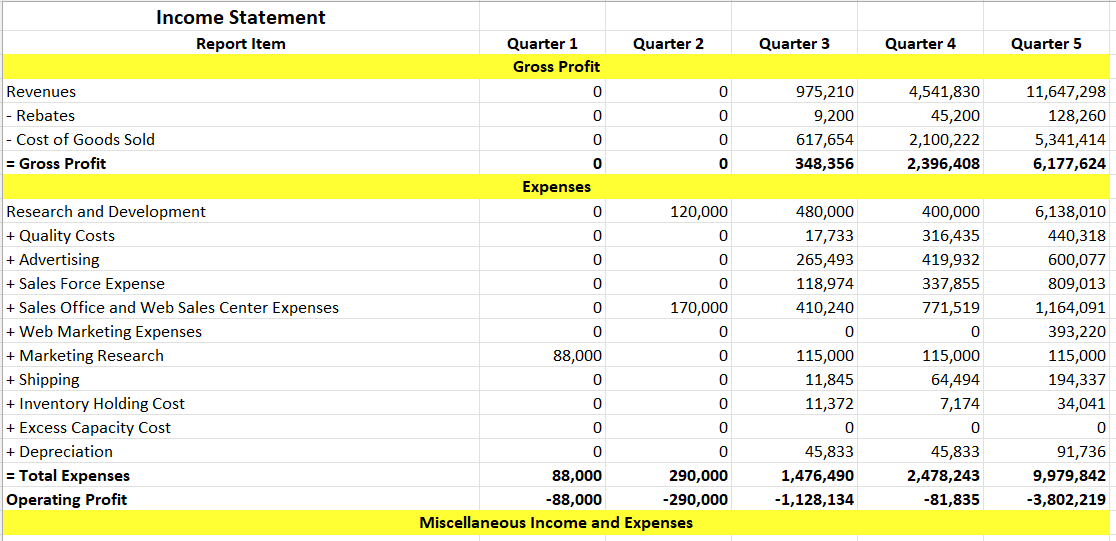
\includegraphics[width=\textwidth]{./img/before}
\caption{Excerto de uma folha de cálculo recebida}
\end{figure}

\begin{figure}[H]
\centering
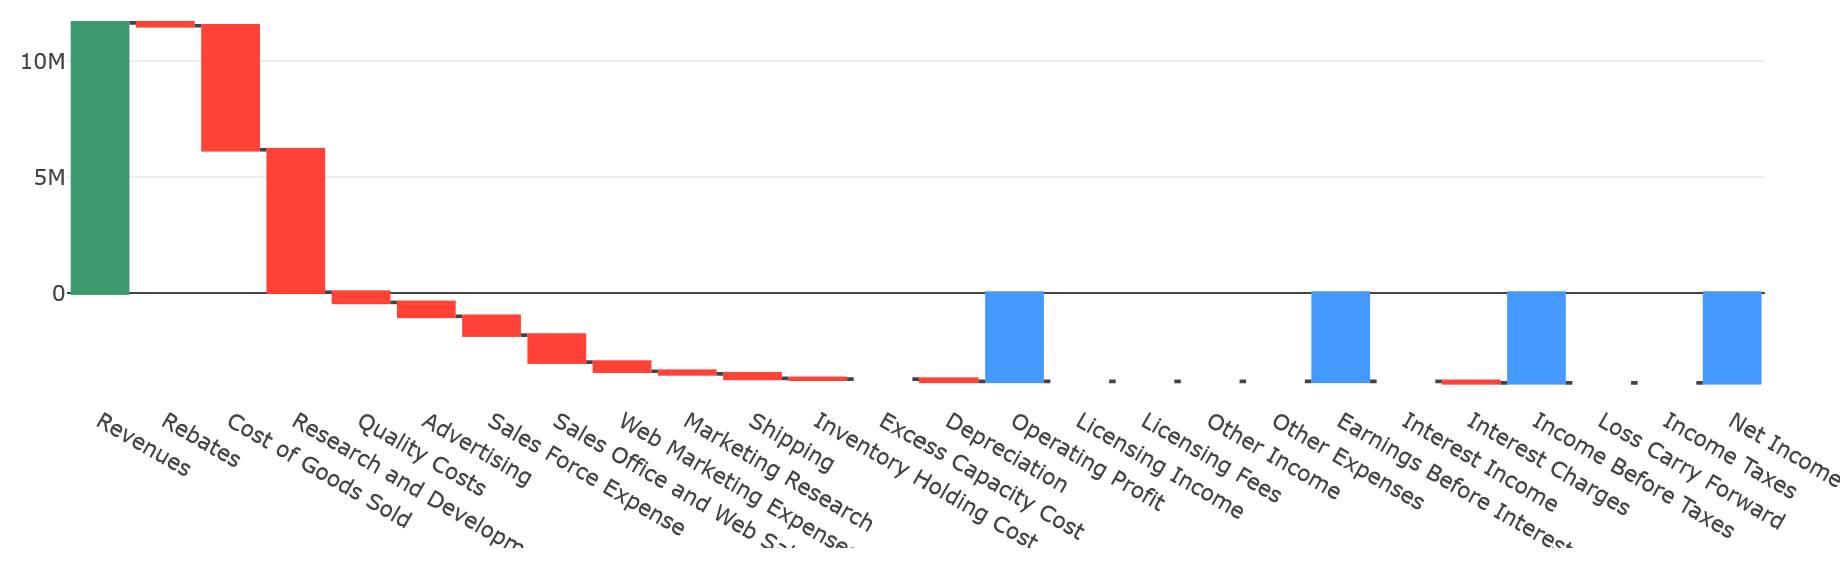
\includegraphics[width=\textwidth]{./img/after}
\caption{Gráfico extraido da mesma folha acima com filtro aplicado para o Quarter 5}
\end{figure}

\section{Desenvolvimento da Aplicação Web}

Esta secção foca-se na estrutura e funcionamento da aplicação web, tanto o backend em Django como a interface construída com HTML, WebComponents e Flowbite.

\subsection{Arquitetura da aplicação (Backend)}

A aplicação web foi desenvolvida utilizando o framework Django como já descrito na secção \ref{sec:fundamentos}. A arquitetura foi desenhada para garantir o isolamento dos dados por utilizador e uma gestão dos ficheiros e dados processados.

\subsubsection{Modelos de Dados}

A aplicação utiliza três modelos principais para gerir os dados, cada um com um papel específico na gestão e organização da informação. Estes modelos formam a base da aplicação, permitindo uma estrutura clara e organizada dos dados.

TODO: Incluir aqui um diagrama de classes com os modelos de dados e as relações entre eles.

\begin{itemize}
    \item \textbf{Quarter:} Representa um trimestre específico para um utilizador. Cada \textit{quarter} tem:
    \begin{itemize}
        \item Um número único por utilizador
        \item Uma precisão configurável para valores numéricos (por omissão 9 casas decimais)
        \item Um UUID único para identificação
        \item Relação com o utilizador que o criou
    \end{itemize}

    \item \textbf{ExcelFile:} Representa um ficheiro Excel carregado para um \textit{quarter} específico:
    \begin{itemize}
        \item Armazena o ficheiro físico em pastas organizadas por UUID
        \item Mantém o estado de processamento (processado/não processado)
        \item Guarda metadados como a secção do ficheiro
        \item Relaciona-se com o \textit{quarter} e o utilizador
    \end{itemize}

    \item \textbf{CSVData:} Armazena os dados processados de cada folha do Excel:
    \begin{itemize}
        \item Guarda os dados em formato \gls{json}
        \item Mantém a ordem original das colunas
        \item Controla qual versão dos dados está ativa
        \item Relaciona-se com o ficheiro Excel de origem e o utilizador
    \end{itemize}
\end{itemize}

\subsubsection{Gestão de Utilizadores}

A aplicação utiliza o mecanismo de utilizadores que já vem incluido com o Django. Este sistema oferece uma camada de segurança, garantindo que apenas utilizadores autenticados possam aceder aos dados. A autenticação na aplicação é feita através de nome de utilizador e palavra-passe e as sessões são geridas pelo Django.

Para garantir a segurança dos dados, todas as rotas que requerem autenticação estão decoradas com \texttt{@login\_required}. Além disso, a aplicação isola dados dados por utilizador, garantindo que cada utilizador só pode aceder aos seus próprios. Este isolamento é implementado através de filtros nas pesquisas, que são aplicados automaticamente em todas as operações de leitura e escrita que são feitas.

Os utilizadores podem criar conta na aplicação, sendo que podem criar conta para si ou para um grupo de utilizadores. A aplicação não faz distinção entre uma conta para um utilizador ou para uma conta para multiplos utilizadores.

\subsubsection{Gestão de Ficheiros e Processamento de dados}

Para conseguirmos manter vários ficheiros em disco, tivemos de pensar num mecanismo capaz de manter ficheiros organizados. Para isso, desenvolvemos um sistema que garante que os dados carregados pelos utilizadores não só ficam protegidos e organizados. Em vez de depender apenas do nome do ficheiro (o que podia facilmente gerar conflitos ou sobreposições), o sistema cria automaticamente uma pasta associada a um UUID, o que garante que cada ficheiro fica isolado do resto. Isto evita situações em que dois ficheiros com nomes iguais se sobrepõem e, ao mesmo tempo, facilita bastante a estruturação interna por quarter, utilizador, ou qualquer outra lógica que venha a ser implementada. Assim que o ficheiro é carregado, o processamento é iniciado, sem depender de passos manuais , ou seja, o utilizador só precisa de fazer o upload e o resto é tratado pelo sistema.

Para além disso, o sistema guarda registos de todos os ficheiros carregados. Quando se carrega um novo ficheiro para substituir outro com o mesmo nome ou que resulta nos mesmos dados, o sistema não apaga o anterior. Em vez disso, marca-o como não atual, processa o novo, atualiza os dados relevantes na base de dados, e mantém o anterior guardado. Esta versão antiga pode ser usada mais tarde, caso seja necessário recuperar informação, validar alterações ou simplesmente reverter um erro. Não foi uma funcionalidade pensada para ser exposta diretamente ao utilizador, e não faz parte do uso normal, mas surgiu como consequência da arquitetura escolhida (ficheiros correntes e não correntes).

\subsubsection{Endpoints para comunicação com o frontend}

A aplicação expõe uma série de endpoints \textit{rest} que permitem a interação com o frontend. Estes endpoints são organizados de forma lógica, com rotas específicas para diferentes funcionalidades. A API inclui endpoints para gestão de \textit{quarters} (\texttt{/api/\textit{quarters}/}) e visualização de gráficos (\texttt{/api/chart/})  O endpoint para visualização de gráficos é o mais importante, e é o que é utilizado para mostrar os gráficos na aplicação web, e permite uma série de parâmetros para filtrar os dados e mostrar gráficos de diferentes tipos. 

Quando a aplicação carrega, não mostra logo todos os gráficos, mas sim um \textit{skeleton} que depois é substituido pelos gráficos, permitindo uma melhor experiência do utilizador. Esse carregamento é feito de forma assincrona, por Javascript, e utiliza o endpoint para visualização de gráficos para obter a configuração final de um gráfico especifico a ser mostrado. A configuração retornada é especifica para a biblioteca Plotly, que depois, juntamente com o restante código Javascript, consegue mostrar o gráfico e aplicar filtros com base nos parâmetros passados.

A comunicação com o backend é feita através de chamadas assíncronas aos \textit{endpoints} desenvolvidos, passando parâmetros como o \textit{quarter} selecionado e os filtros ativos. O backend devolve a estrutura necessária para renderização com Plotly, assegurando que cada gráfico é gerado com os dados e configurações corretas.

\subsection{Interface Gráfica (Frontend)}

A interface da aplicação foi desenhada com foco na usabilidade e consistência visual, através da utilização de tecnologias modernas como WebComponents e através de um design system, Flowbite. O objetivo era garantir uma experiência responsiva, adequada para desktop e que suportasse minimamente dispositivos móveis, sem comprometer a performance nem a clareza na apresentação dos dados.

\subsubsection{Design System com Flowbite}

A escolha do Flowbite, assente sobre Tailwind CSS, permitiu acelerar o desenvolvimento com componentes reutilizáveis e visualmente consistentes. Esta abordagem simplificou a criação de elementos como modais, formulários, botões entre outros elementos, garantindo uma interface limpa e padronizada. A navegação é feita através de uma barra lateral com todas as secções disponiveis, enquanto modais são usados para operações críticas como confirmações e carregamento de ficheiros. A coerência visual é reforçada por tipografia, cores e espaçamentos, permitindo aos utilizadores focarem-se na análise sem distrações.

\subsubsection{WebComponents}

A camada de visualização de dados é composta por componentes Web personalizados, cada um encapsulando a lógica de um tipo específico de gráfico. Esta abordagem modular garante isolamento entre componentes, facilita a reutilização e simplifica a manutenção do código Javascript. Na prática, a especificação WebComponents\cite{webcomponents} permite criar os nossos nós DOM, e estende as interfaces DOM já existentes. Esta funcionalidade permite criar componentes que se comportam como elementos HTML, e que podem ser utilizados como tal, e que também podem receber estilos e outras propriedades e atributos e é suportada já pelos os browsers mais usados (como pode ser consultado no site Can I Use\cite{caniuse} que é um site que consegue consultar o suporte de uma funcionalidade em diferentes browsers).

\begin{figure}[H]
    \centering
    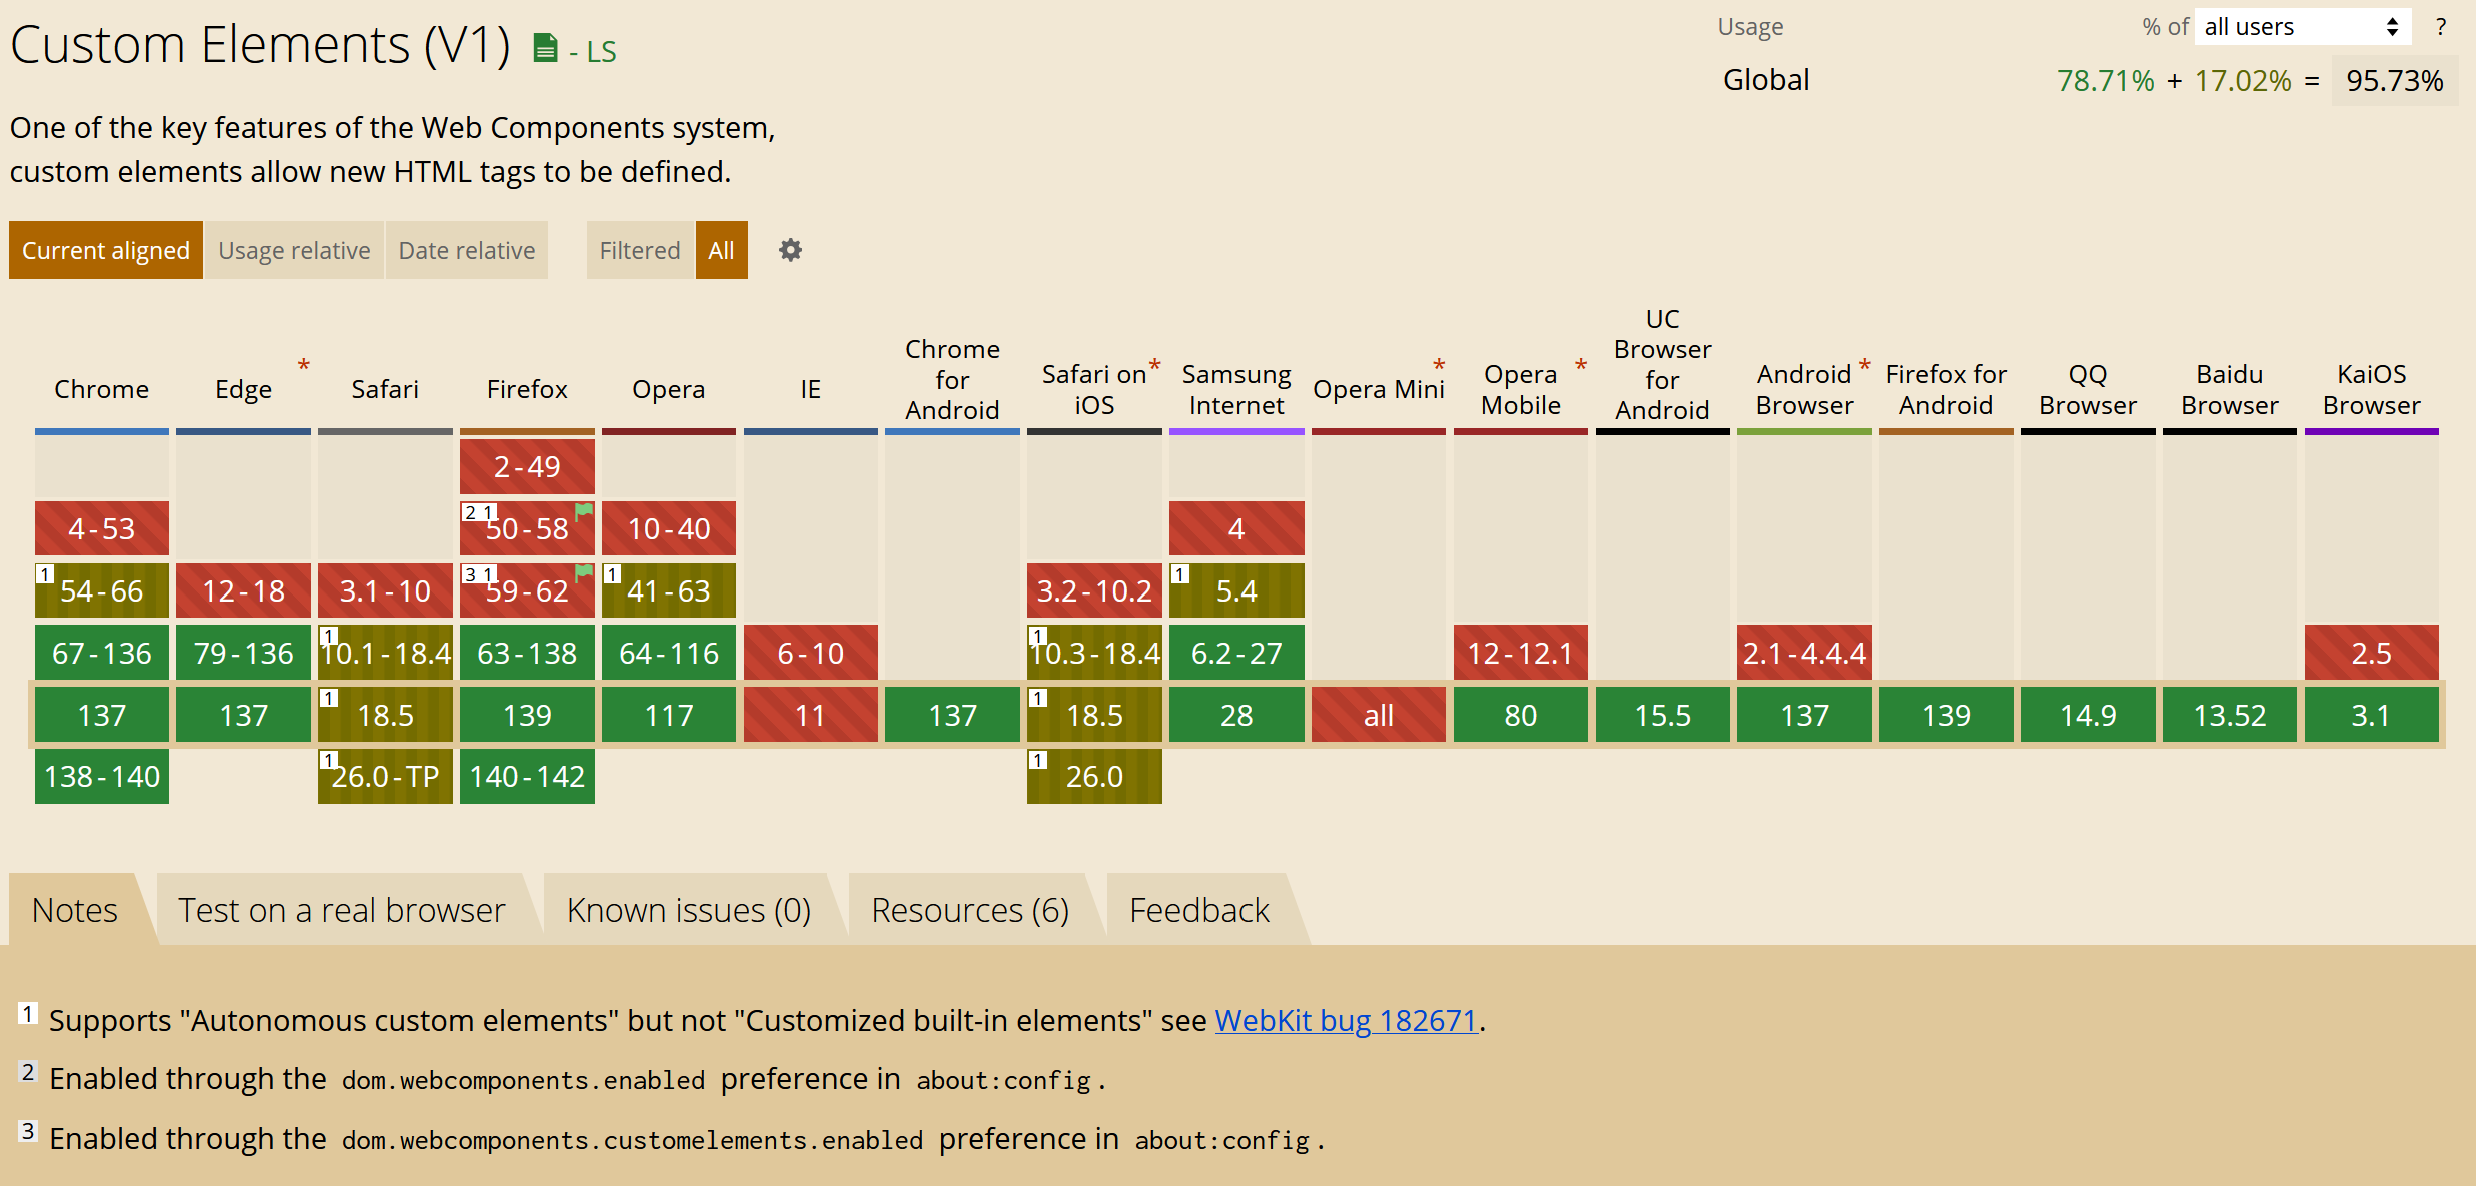
\includegraphics[width=\textwidth]{./img/caniuse}
 \caption{Suporte de WebComponents em navegadores}
 \end{figure}


Na nossa aplicação, os WebComponents são usados como elementos HTML normais, que recebem apenas o gráfico que é para mostrar. Ao carregar, fazem uma chamada a um \textit{endpoint} do backend, que retorna a configuração do gráfico, e que é utilizada para mostrar o gráfico.

\begin{figure}[H]
    \centering
    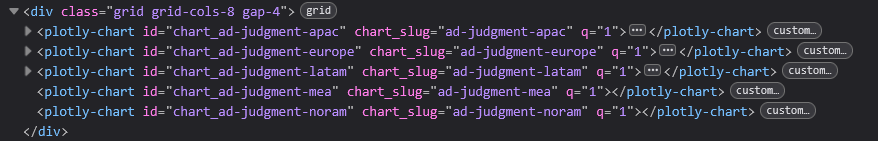
\includegraphics[width=\textwidth]{./img/webc}
 \caption{Utilização de WebComponents na aplicação}
 \end{figure}

A comunicação com o backend é feita através de chamadas assíncronas aos \textit{endpoints} desenvolvidos, passando parâmetros como o \textit{quarter} selecionado e os filtros ativos. O backend devolve a estrutura necessária para renderização com Plotly, assegurando que cada gráfico é gerado com os dados e configurações corretas. Os gráficos são carregados de forma progressiva, com um \textit{skeleton} que é substituido pelo gráfico quando os dados estão prontos, e apenas são mostrados quando entram dentro do \textit{viewport} do utilizador (\textit{lazy load}). O \textit{lazy load} permite que os servidor não fique sobre-carregado com pedidos, e que no lado do cliente, a memória utilizada seja minimizada visto que não são carregados todos os gráficos de uma vez.	

As bibliotecas Plotly e Datatables foram integradas diretamente com os WebComponents\cite{webcomponents}, fazendo com que o WebComponent consiga mostrar gráficos e tabelas de forma encapsulada. Esta integração permite também que o carregamento seja feito de forma progressiva em cada gráfico é inicialmente substituído por um \textit{skeleton} (uma representação visual com um \textit{spinner} e com a largura e altura aproximada de um gráfico) que desaparece quando os dados ficam disponíveis. A ideia deste \textit{skeleton} é que o utilizador veja que o gráfico está a ser carregado, e que não cause um grande deslocamento do gráfico na interface quando os dados estão prontos.

\subsubsection{Responsividade em dispositivos móveis}

Toda a interface foi pensada para ser utilizada em computadores devido à quantidade de gráficos que são apresentados. A interface adapta-se bem a dispositivos moveis, mas devido ao espaço disponivel, não é possível garantir uma boa experiencia de utilização em dispositivos moveis. A aplicação tem, essencialmente, 2 \textit{media queries}. Uma \textit{media query} que até aos 1023px que inclui telemóveis, tablets e ecrãs pequenos, e uma \textit{media query} a partir dos 1024px que inclui computadores e ecrãs maiores.

\begin{figure}[H]
    \centering
    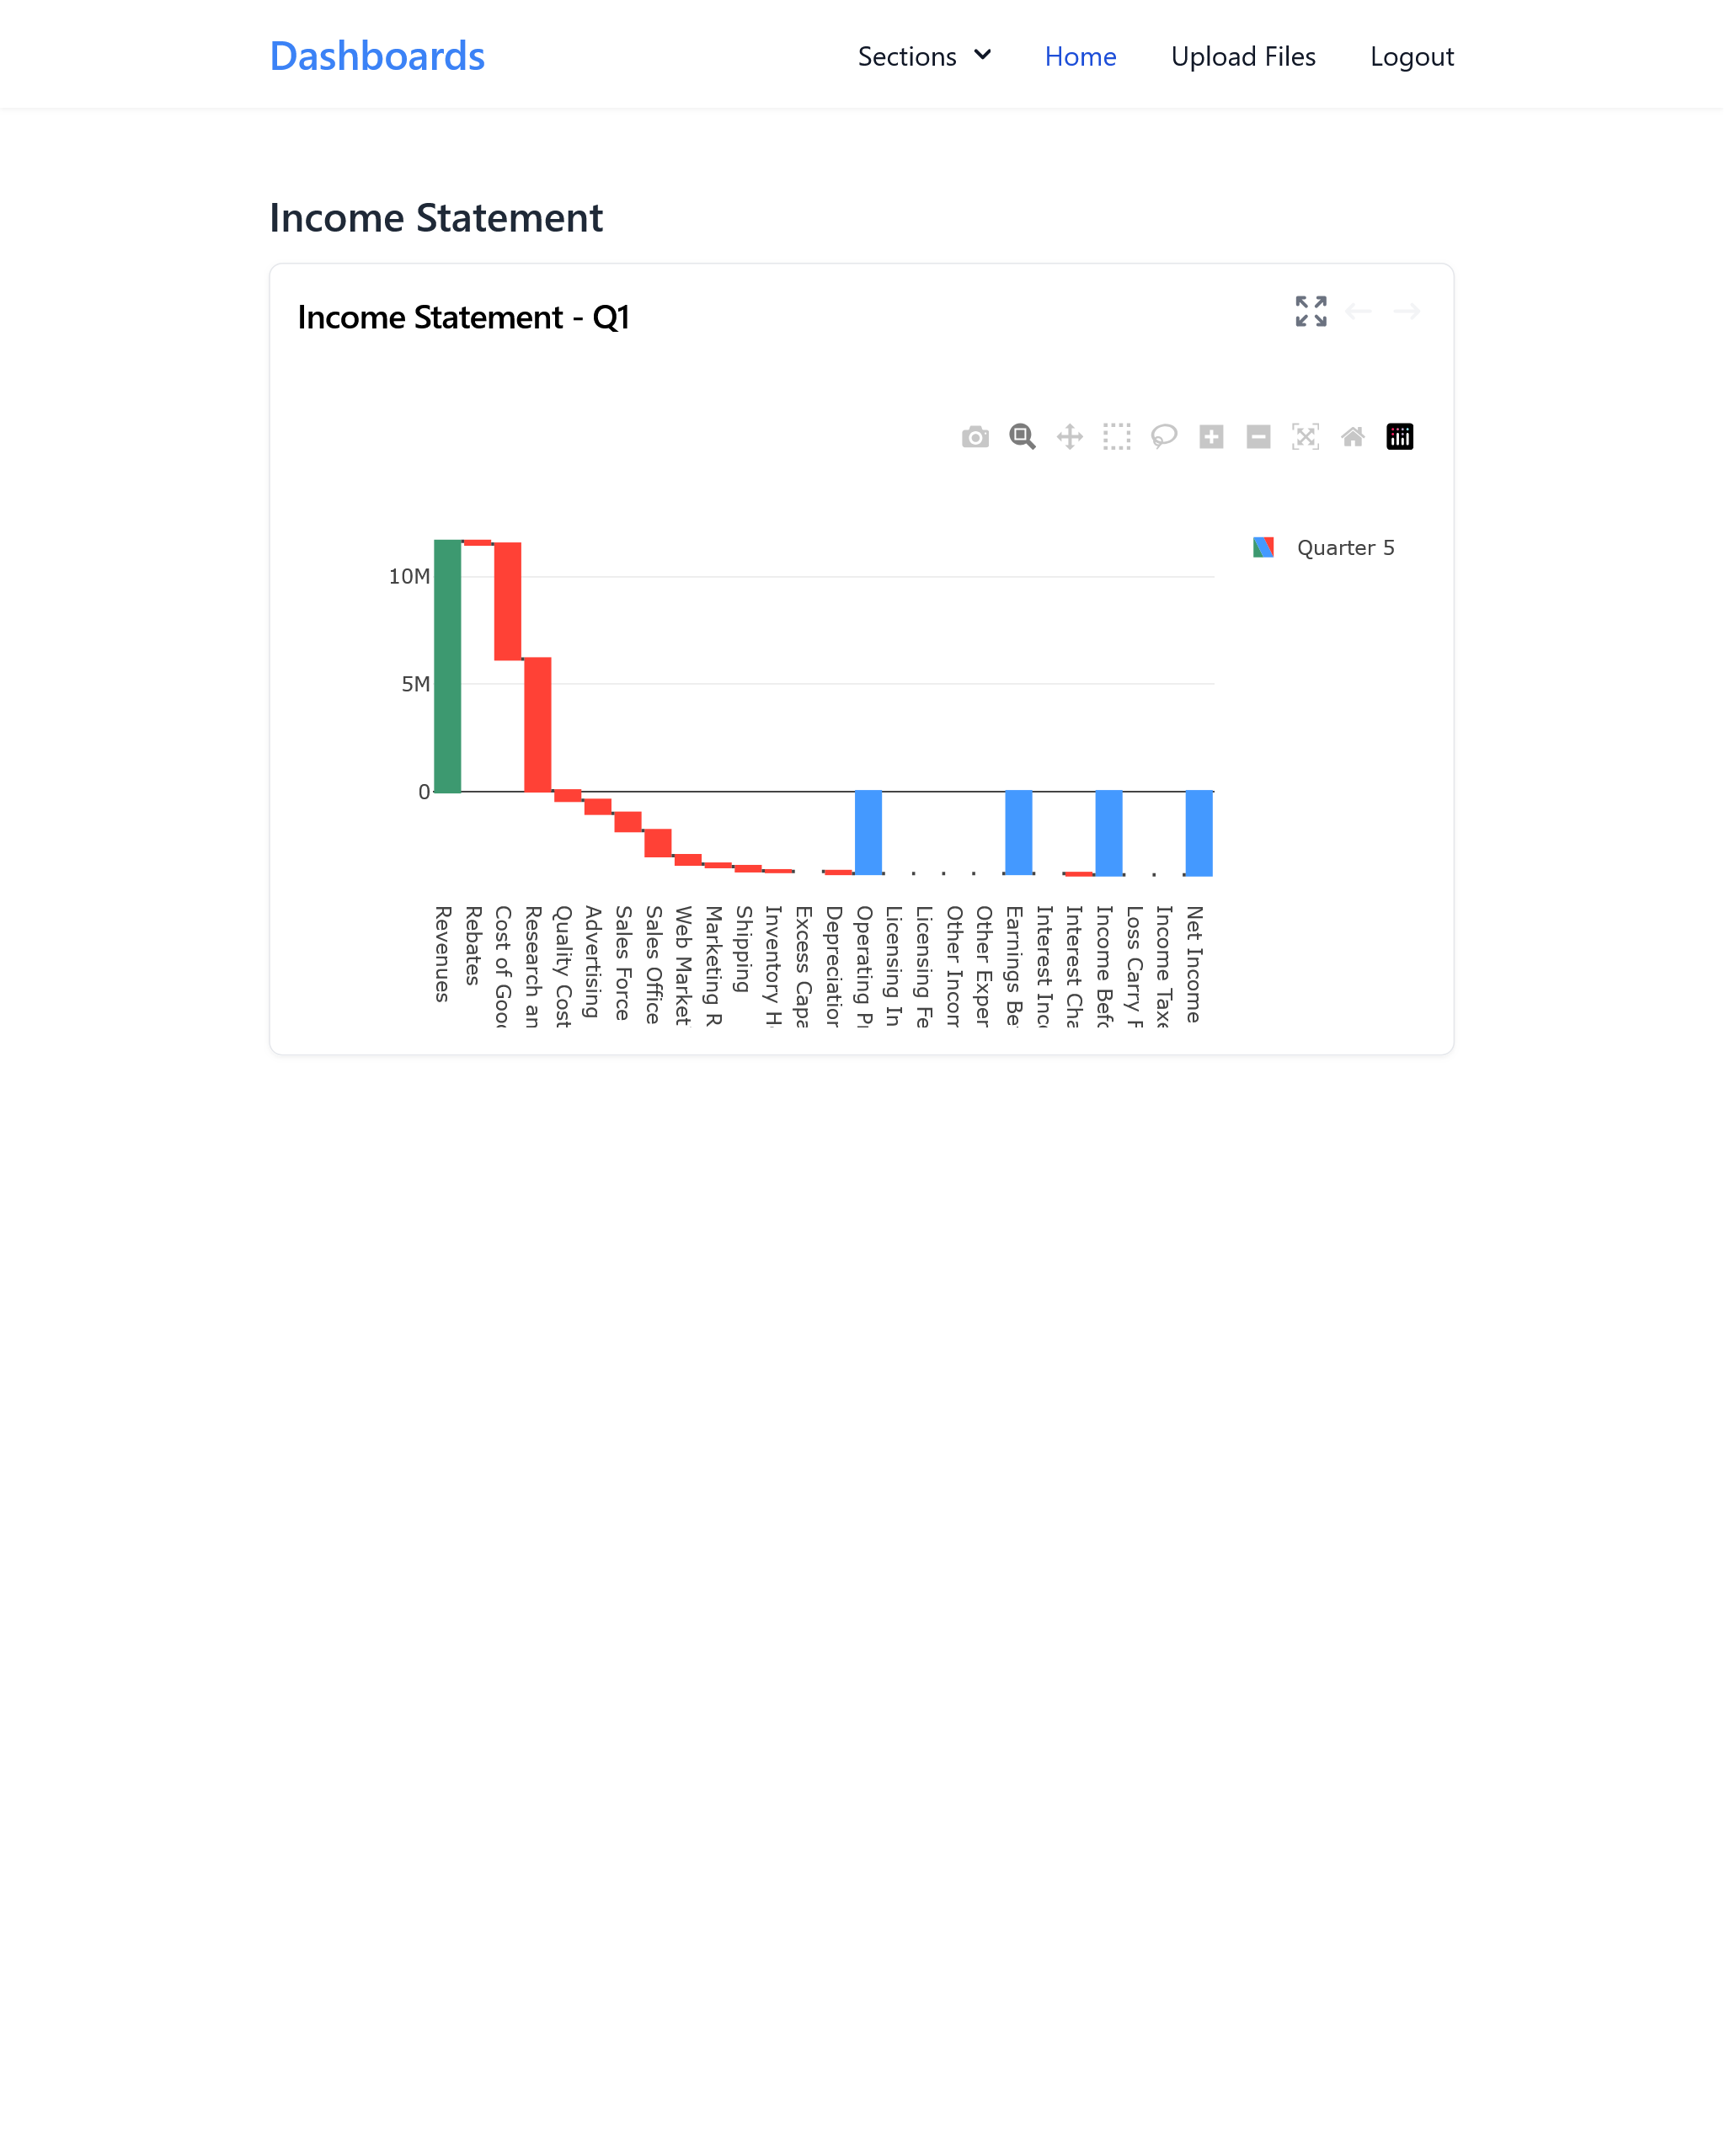
\includegraphics[width=\textwidth]{./img/res_1023}
 \caption{Media query até 1023px}
\end{figure}


\begin{figure}[H]
    \centering
    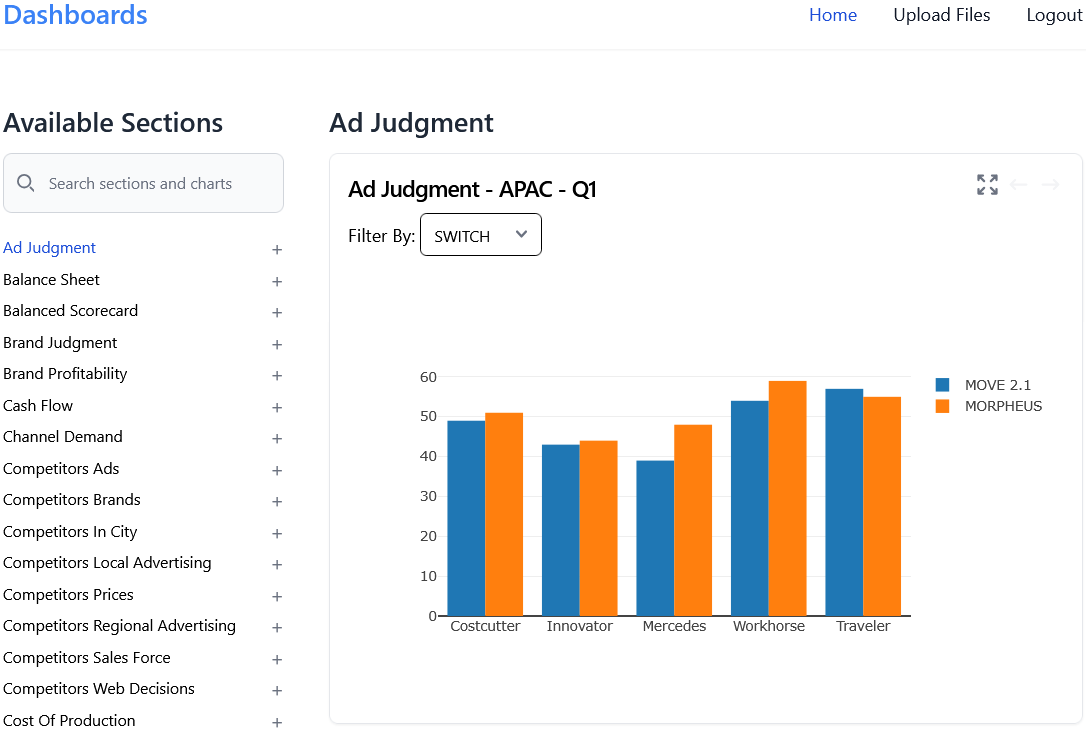
\includegraphics[width=\textwidth]{./img/res_1920}
 \caption{Media query a partir dos 1024px}
\end{figure}

Estes \textit{media queries} são muito utilizados para adaptar a interface aos diferentes tamanhos de ecrã, garantindo uma boa experiência de utilização em todos os dispositivos, sendo que não tivemos de fazer código explicitamente para a aplicação se adaptar para dispositivos móveis. Os filtros dinâmicos permitem ajustar os gráficos em tempo real, com \textit{feedback} visual imediato não sendo necessário recarregar a página. No momento em que o filtro troca, é feito um pedido a API de gráficos que retorna um novo conjunto de dados para mostrar, com a configuração do gráfico atualizada.

\subsubsection{Carregamento de ficheiros}

A organização dos dados foi pensada para refletir a lógica do projeto Marketplace Simulations. Cada utilizador pode criar múltiplos \textit{quarters} no momento em que carrega um ficheiro. Estes \textit{quarters} funcionam como buckets isolados onde são armazenados os ficheiros carregados. A navegação entre \textit{quarters} é facilitada por setas laterais em cada gráfico apresentado. A criação e remoção de \textit{quarters}, bem como o carregamento de ficheiros, é acompanhada por feedback visual no momento da ação.

Para verificar se os ficheiros são do tipo correto, decidimos validar através do \textit{MIME type}, que é um identificador padronizado utilizado para descrever o tipo de conteúdo de um ficheiro. Os \textit{MIME types} seguem o formato \texttt{tipo/subtipo}, como por exemplo \texttt{text/csv} para ficheiros CSV ou \texttt{application/vnd.openxmlformats-officedocument.spreadsheetml.sheet} para ficheiros Excel no formato \texttt{.xlsx}. Esta abordagem permite garantir que os ficheiros carregados correspondem realmente ao formato esperado, independentemente da extensão do nome do ficheiro, que pode ser facilmente manipulada. Ao inspecionar o \textit{MIME type} real do conteúdo, conseguimos rejeitar ficheiros inválidos ou maliciosos de forma mais robusta. No contexto deste projeto, esta verificação revelou-se essencial, uma vez que apenas ficheiros \texttt{.xlsx} válidos devem ser processados. Assim, a validação por \textit{MIME type} contribui tanto para a segurança como para a integridade do sistema.

Durante o carregamento, a interface valida se os ficheiros são do tipo correto. Apenas ficheiros dos mime type \texttt{application/vnd.openxmlformats-officedocument.spreadsheetml.sheet} e \texttt{application/vnd.ms-excel} são permitidos. Quando um ficheiro com o mesmo nome é enviado, este não sobrescreve o anterior,  mas é marcado os ficheiros antigos como não correntes. Uma outra funcionalidade é a resiliencia a ficheiros maliciosos. No nosso caso, a biblioteca Pandas não permite a execução de código, pelo que não é possivel executar código malicioso que seja incluido nos ficheiros. 

%%________________________________________________________________________
\chapter{Validação e Testes}
\label{ch:validacaoTestes}
%%________________________________________________________________________

A validação e testes da aplicação foram realizados através de múltiplas abordagens, garantindo uma cobertura de testes  da funcionalidade como da usabilidade da aplicação. Este capítulo descreve as diferentes estratégias de teste implementadas e os resultados obtidos.

\section{Testes de Acessibilidade}

A acessibilidade foi uma preocupação no desenvolvimento da aplicação, e para isso foram seguidas as diretrizes \gls{wcag} 2.1, que definem critérios técnicos para tornar os conteúdos web mais acessíveis a todos os utilizadores, incluindo pessoas com deficiências visuais, motoras, auditivas, cognitivas ou neurológicas. Para garantir a conformidade com estas diretrizes, recorremos a uma abordagem prática combinada de testes automáticos e validação manual. Entre as ferramentas utilizadas destacam-se duas principais: o Lighthouse e o Axe.

O Lighthouse, desenvolvido pela Google, é uma ferramenta open source que corre diretamente no Chrome DevTools ou como \gls{cli}. Permite auditar uma página web em várias categorias, nomeadamente Performance, SEO, Best Practices e, claro, Accessibility. A secção de acessibilidade do Lighthouse verifica, por exemplo, se os elementos têm contrastes suficientes, se os formulários estão corretamente identificadas com atributos aria-label, se há títulos estruturados (h1, h2, etc.) numa hierarquia lógica e se os elementos interativos (como botões e links) são acessíveis por teclado. O Lighthouse fornece uma pontuação de 0 a 100 e destaca problemas comuns com sugestões de como resolver.

Esta ferramenta Lighthouse, apesar de não ser tão detalhada como a Axe, sinalizou alguns problemas, como a falta de compressão \gls{gzip} e alguns erros de acessibilidade e \gls{seo}. Estes problemas foram resolvidos (fazendo alterações na configuração do servidor Nginx e no código da aplicação), e a ferramenta Lighthouse passou a dar uma pontuação melhor nos vários critérios que avalia.

\begin{figure}[H]
\centering
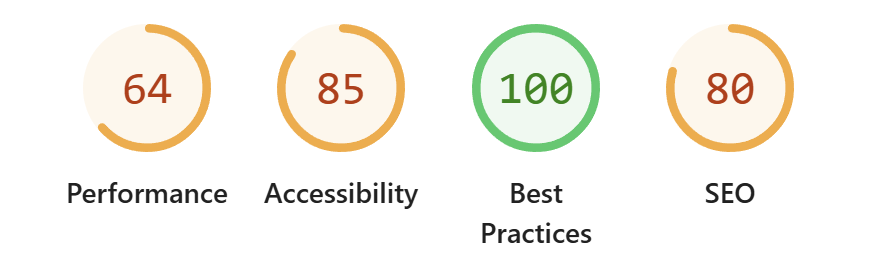
\includegraphics[width=\textwidth]{./img/lh_before}
\caption{Testes de acessibilidade com a ferramenta Lighthouse}
\end{figure}

\begin{figure}[H]
\centering

\includegraphics[width=\textwidth]{./img/lh_after}
\caption{Testes de acessibilidade com a ferramenta Lighthouse após as correções}
\end{figure}

Já o Axe, da empresa Deque, é uma biblioteca de testes de acessibilidade mais focada, muito utilizada em ambientes de desenvolvimento profissional. Pode ser usada como extensão do browser ou integrada com ferramentas de testes automatizados como Cypress ou Selenium. O Axe segue os critérios \gls{wcag} com mais profundidade e reporta violações como a ausência de nomes acessíveis (\textit{accessible names}), uso incorreto de landmarks \gls{aria}, falhas de foco, ou elementos visuais sem correspondência textual. Além disso, o Axe permite navegar entre os erros diretamente na interface do browser, o que torna o processo de debugging muito mais fácil.

Nos primeiros testes feitos com a ferramenta Axe, as ferramentas sinalizaram alguns problemas relativos a acessibilidade, como a falta de textos alternativos para alguns elementos visuais, e os niveis dos titulos não estavam a ser usados de forma adequada.

\begin{figure}[H]
    \centering
    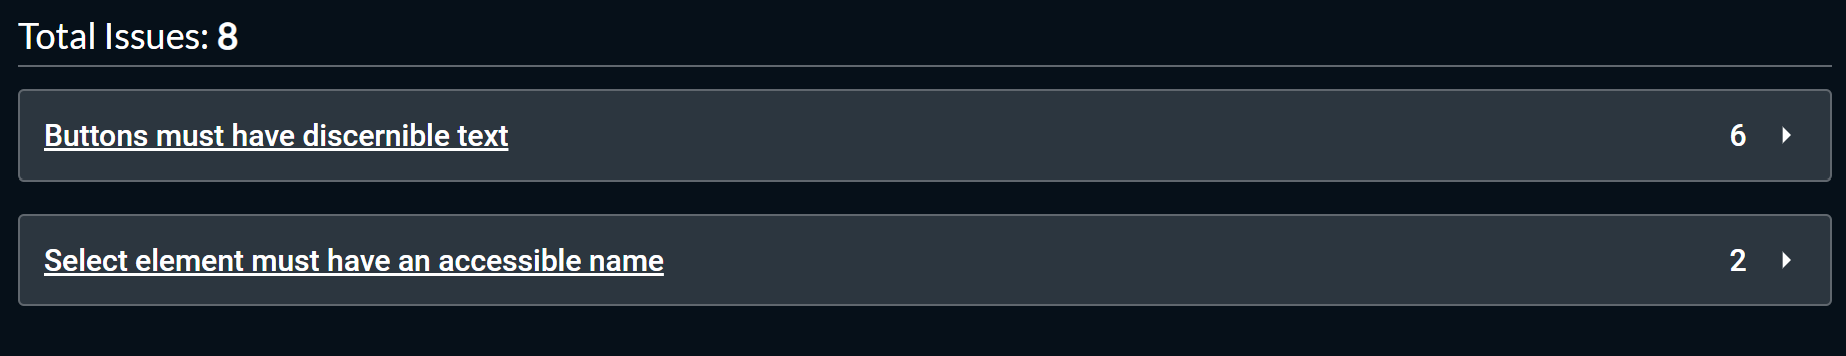
\includegraphics[width=\textwidth]{./img/axe}
    \caption{Testes de acessibilidade com a ferramenta Axe}
    \end{figure}


Após resolver os problemas indicados pela ferramenta Axe, conseguimos então melhorar a acessibilidade da aplicação, como se pode ver na imagem abaixo.

\begin{figure}[H]
\centering
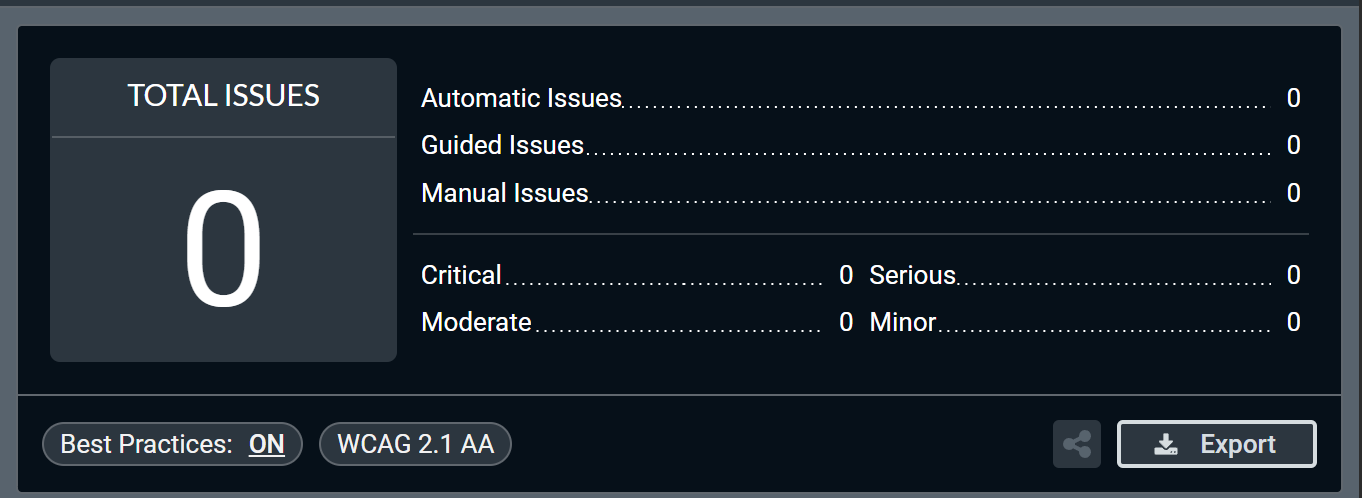
\includegraphics[width=\textwidth]{./img/axe_after}
\caption{Testes de acessibilidade com a ferramenta Axe após as correções}
\end{figure}

No nosso caso, ambas as ferramentas foram utilizadas de forma complementar: o Lighthouse ajudou-nos a identificar problemas mais genéricos e dar uma visão rápida do estado da acessibilidade da aplicação, enquanto o Axe foi essencial para validar critérios mais técnicos e detetar problemas complexos que o Lighthouse pode não cobrir. Os testes foram feitos tanto em páginas com dados carregados como em estados vazios, e procurámos garantir que todas as interações essenciais da plataforma,  como o Carregamento de ficheiros, usabilidade e navegação entre gráficos fossem utilizáveis por utilizadores com leitores de ecrã e navegação apenas por teclado.

Desta forma, procurámos alinhar a aplicação com boas práticas de desenvolvimento inclusivo, respeitando não só normas técnicas mas também a responsabilidade social de criar interfaces acessíveis a todos, com foco nas seguintes funcionalidades:
\begin{itemize}
    \item Adição de textos alternativos para todos os elementos visuais
    \item Garantia de contraste adequado entre texto e fundo
    \item Implementação de navegação por teclado
    \item Estruturação semântica de \gls{html}
    \item Suporte a leitores de ecrã
\end{itemize}

\section{Testes Manuais}

Para complementar os testes automatizados, foi desenvolvido um conjunto abrangente de testes manuais utilizando a linguagem Gherkin para descrever os cenários de teste. Gherkin é uma linguagem estruturada, mas legível por humanos, que permite descrever comportamentos esperados do sistema em forma de cenários do tipo Dado-Quando-Então. Esta abordagem facilita a comunicação entre equipas técnicas e não técnicas, garantindo que todos os intervenientes compreendam os objetivos de cada teste.

Foi pedido a cinco testadores independentes para executarem estes testes manualmente, com base nos cenários escritos em Gherkin, e no final preencherem um formulário com os resultados de cada execução, incluindo observações e eventuais desvios face ao comportamento esperado. Os cenários de teste foram organizados em duas categorias principais:

\begin{itemize}
    \item Fluxos de utilizador (criação de conta, login, navegação)
    \item Operações com dados (carregar e apagar ficheiros, visualização de gráficos)
\end{itemize}

Cada cenário foi documentado usando a sintaxe Gherkin, permitindo uma clara compreensão dos pré-requisitos, ações e resultados esperados, como exemplificado abaixo. Os restantes cenarios Gherkin irão ser incluidos em anexo.

\begin{verbatim}
Scenario: Creating an account
	Given I access the page 
	And I don't have an account or logged in
	Then I should see the "Create Account" link
	When I click the "Create Account" link
	Then I should be redirected to the "Create Account" form
	And I should see the username field
	And I should see the password filed
	And I should see the confirm password field
	When I fill that form
	And I click "Save"
	Then I should be redirected to the "Login" page
\end{verbatim}

Os restantes cenários Gherkin foram incluídos no apêndice \ref{ch:cenariosGherkin}.

Apesar desta amostra não ser muito representativa, foi possivel encontrar bugs na aplicação, como por exemplo, a falta de alguns dados em alguns gráficos, e alguns gráficos náo serem coerentes com a informação que estavam a mostrar. Estes bugs foram corrigidos assim que foram reportados pelos testadores.

TODO: Falta falar sobre a análise dos resultados dos testes manuais.

\section{Compatibilidade com Navegadores}

A compatibilidade com diferentes navegadores foi testada utilizando a plataforma BrowserStack, que permitiu testar a aplicação em múltiplos ambientes. Os testes foram realizados nas versões mais recentes dos principais navegadores:

\begin{itemize}
    \item Google Chrome (versões 90+)
    \item Mozilla Firefox (versões 88+)
    \item Microsoft Edge (versões 90+)
    \item Safari (versões 14+)
\end{itemize}

A aplicação demonstrou compatibilidade com os navegadores testados, com exceção do Internet Explorer 11, que não é suportado devido a limitações técnicas e à baixa utilização atual deste navegador.

Os testes de compatibilidade incluíram:
\begin{itemize}
    \item Renderização correta de todos os componentes
    \item Funcionalidade completa de todos os recursos
    \item Comportamento consistente em diferentes resoluções
    \item Suporte a recursos modernos do JavaScript
\end{itemize}

\section{Conclusões dos Testes}

Os resultados dos diferentes tipos de testes realizados permitiram identificar e corrigir várias questões antes do lançamento da aplicação. As principais conclusões foram:

\begin{itemize}
    \item Alta pontuação em acessibilidade, demonstrando o compromisso com a inclusão digital
    \item Boa performance geral, com tempos de resposta adequados
    \item Compatibilidade robusta com navegadores modernos
    \item Interface intuitiva e fácil de usar, conforme validado pelos testes manuais
\end{itemize}

Estas validações confirmaram que a aplicação atende aos requisitos estabelecidos no capítulo \ref{ch:modeloProposto}, particularmente em relação aos fundamentos técnicos descritos na secção \ref{sec:fundamentos}.

%%________________________________________________________________________
\chapter{Conclusões e Trabalho Futuro}
\label{ch:conclusoesTrabalhoFuturo}
%%________________________________________________________________________

O desenvolvimento deste projeto culminou numa aplicação web funcional que responde de forma direta e eficaz às necessidades dos estudantes do ISCAL no que diz respeito à análise dos dados exportados da plataforma Marketplace Simulations. Desde o início, o objetivo foi construir uma solução prática, que facilitasse a leitura e exploração da informação, e ao mesmo tempo fosse suficientemente robusta e escalável para crescer com os utilizadores e os dados.

\section{Conclusões}

Um dos pontos fortes deste projeto foi a implementação de um sistema automático para gerir ficheiros e transformar dados em gráficos. Esta funcionalidade, de os utilizadores poderem carregar ficheiros diretamente exportados do simulador e, a partir daí, obterem gráficos interativos, sem qualquer necessidade de formatação manual representa uma melhoria relação ao processo anterior, que era manual, demorado e propenso a erros. 

A decisão de usar Django como base para o backend revelou-se acertada. Além de facilitar a autenticação e gestão de utilizadores, a  biblioteca permitiu implementar uma boa arquitetura, com separação entre as camadas frontend e backend. A autenticação integrada, associada ao isolamento de dados por utilizador, garantiu uma camada extra de segurança sem complicar a lógica da aplicação. A API REST que foi construída permitiu uma comunicação fluida entre as várias partes do sistema, suportando atualizações dinâmicas dos gráficos sem impacto na performance.

No lado do frontend, optou-se por uma abordagem prática, usando bibliotecas para garantir a responsabilidade e usabilidade. A biblioteca Plotly foi fundamental para criar gráficos interativos que, além de apelativos, ajudam os estudantes a interpretar os dados.

Durante o desenvolvimento surgiram alguns desafios técnicos. Um dos principais foi lidar com a diversidade estrutural dos ficheiros. Alguns traziam folhas com formatação irregular, nomes de colunas inconsistentes ou dados dificeis de perceber. Isso obrigou à criação de uma pipeline de normalização robusto e reutilizável que é uma componente essencial para garantir que os dados fossem processados corretamente e de forma previsível. Apesar da solução atual funcionar bem no contexto do projeto, poderá ser necessário alterar no futuro caso os ficheiros evoluam ou incluam novos tipos de dados. Outro ponto que pode ser melhorado é a interface de gestão de \textit{quarters}, que embora funcional, ainda exige alguma familiaridade com o conceito por parte do utilizador.

Para além do lado técnico, este projeto foi também uma excelente oportunidade de crescimento pessoal. Antes de começar, não tinha experiência prática com Django nem com bibliotecas como Pandas, e o contacto com estas tecnologias acabou por ser fundamental. Esta aprendizagem provou o valor da adaptação contínua e da experimentação prática como pilares fundamentais do desenvolvimento de software.

Em síntese, este projeto mostrou como a combinação de ferramentas modernas pode resultar numa solução escalável e com impacto direto na experiência de aprendizagem. A aplicação desenvolvida resolve um problema enfrentado pelos estudantes do ISCAL, e deixa aberta a porta para futuras melhorias e novos casos de uso. É uma base sólida, que pode ser facilmente estendida ou adaptada a outros contextos educacionais onde a análise de dados seja um desafio.

\section{Trabalho Futuro}

Apesar de o sistema atual já cumprir os objetivos definidos inicialmente, foram identificadas diversas oportunidades de evolução e expansão que poderão ser exploradas em futuras iterações do projeto. Estas propostas estão organizadas em diferentes áreas de desenvolvimento.

\subsection{Interface e Experiência do Utilizador}

Uma das direções mais imediatas para evolução está ao nível da interface. Pretende-se alargar o leque de visualizações disponíveis, incluindo novos tipos de gráficos, como dispersões, histogramas ou até mapas interativos, sendo que é sempre importante ter em mente a experiencia de utilização. Para além disso, seria interessante permitir a criação de \textit{dashboards} personalizáveis, onde cada utilizador poderia compor visualizações de acordo com os seus objetivos, e até juntar vários tipos de dados na mesma visualização.

Outro aspeto relevante prende-se com a configuração dinâmica dos gráficos. A ideia é deixar de apresentar visualizações estáticas e passar a oferecer ao utilizador a possibilidade de escolher, em tempo real, os tipos de gráfico, métricas e dimensões que pretende analisar. Esta abordagem aumentaria substancialmente a flexibilidade da ferramenta.

\subsection{Análise de Dados e Otimização de Performance}

Do ponto de vista analítico, uma evolução natural do sistema passa pela incorporação de técnicas de análise preditiva. A utilização de modelos de regressão ou algoritmos de aprendizagem automática simples poderá ajudar os estudantes a identificar padrões e antecipar tendências de mercado com base nos dados da simulação.

Em paralelo, importa melhorar a eficiência do sistema no processamento de dados de maior volume. Será relevante avaliar o uso de bibliotecas como \texttt{Dask} ou \texttt{Polars}, que oferecem soluções otimizadas para manipulação de grandes \textit{datasets}, mantendo tempos de resposta aceitáveis e garantindo uma boa experiência de utilização.

\subsection{Gestão de Utilizadores e Colaboração}

Ao nível da gestão da plataforma, propõe-se o reforço das funcionalidades de administração de utilizadores. Isto poderá incluir a criação de perfis diferenciados (por exemplo, administrador, editor, visualizador) e mecanismos de controlo de permissões.

Adicionalmente, seria interessante introduzir funcionalidades de colaboração entre utilizadores, nomeadamente a partilha de visualizações e filtros de dados. Este tipo de funcionalidade é particularmente útil em contextos académicos, onde os trabalhos são frequentemente realizados em grupo ao longo do semestre.

\subsection{Integração com Outras Plataformas}

Por fim, um caminho a explorar passa pela integração direta com a plataforma \textit{Marketplace Simulations}, de onde os dados são originalmente extraídos. Uma abordagem possível seria o desenvolvimento de extensões de navegador (para \textit{Chrome}, \textit{Firefox} ou \textit{Edge}) que permitam importar automaticamente os dados para o nosso sistema, eliminando etapas manuais do processo de upload.

De forma geral, estas propostas de melhoria mostram que o projeto pode continuar a evoluir significativamente, servindo como base para novas investigações ou aplicações.







